
\documentclass[11pt]{presentation}
% alternativ 14pt or 17pt (von beamer unterstützt)

\veranstaltung{Model Checking for (Modular) Petri Nets}
\dozentin{Sophie Wallner}
\universitaet{University of Rostock}

\mode<presentation>{}

\begin{document}

% Titelseite
{
\usebackgroundtemplate{
	\begin{picture}(0,270)
		\tikz\node[opacity=0.1]{\hspace*{1.4cm}
\includegraphics[width=0.75\paperwidth]{resources/logo.png}};
	\end{picture}}

\begin{frame}[noframenumbering,plain]
	\titlepage
\end{frame}
}

\section{Model Checking}

\begin{frame}[noframenumbering,plain]{Section Page}
	\sectionpage
\end{frame}

\begin{frame}{General}
	Computer-aided Verification Method \cite{clarke_automatic_1986}

	\bigskip
	$ \rightarrow $ Evaluate behavior of a system

	\bigskip
	$ \not = $ Testing

	\bigskip
	Fields of Application
	\begin{itemize}
		\item Safety-critical systems (traffic, aviation, medical devices, etc.)
		\item Mission-critical systems (extensive testing not possible, e.g., spaceflight)
	\end{itemize}
	{\centering
	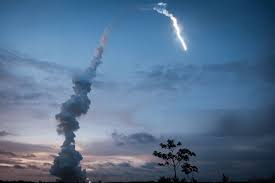
\includegraphics[width=0.4\textwidth]{resources/ariane5.jpeg}
	\par}

\end{frame}

\begin{frame}{Model Checking Pipeline}
	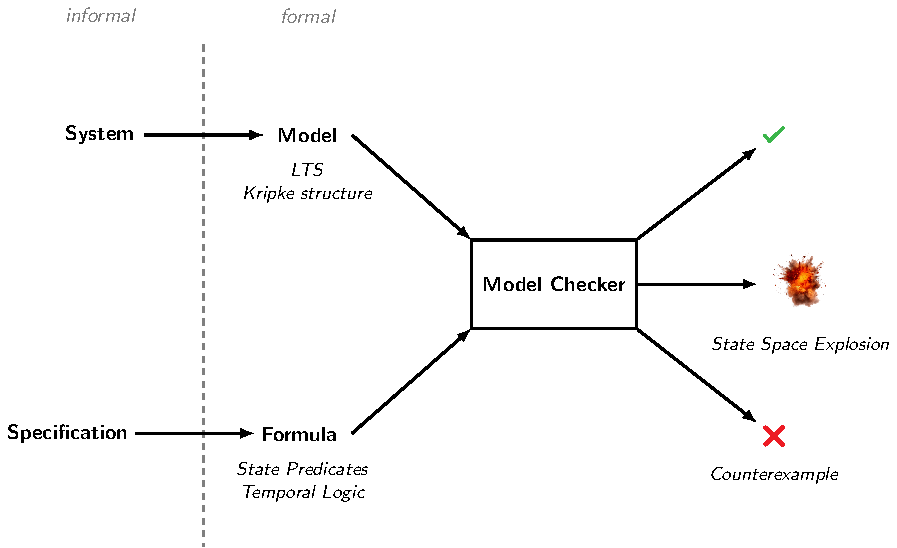
\includegraphics[width=\textwidth]{resources/pipeline.pdf}
\end{frame}

\section{Petri Nets}

\begin{frame}[noframenumbering,plain]{Section Page}
	\sectionpage
\end{frame}

\begin{frame}{General}
	Modeling formalism for discrete Systems

	\medskip
	Causality and concurrency can be easily illustrated

	\medskip
	\begin{defi}{Petri Net, Marking \cite{desel_placetransition_1996}}{}
		A \emph{Petri net} is a tuple $ N = [P,T,f,w,\marking[0]] $:
		\begin{itemize}
			\item $ P $ --  finite set of \emph{places}
			\item $ T $ -- finite set of \emph{transitions} with $ P \cap T = \emptyset $
			\item $ f \subseteq (P \times T) \cup (T \times P) $ -- \emph{flow relation}
			\item $ w : f \rightarrow \nat \setminus \set{0} $ -- \emph{weight function}
			\item  $ \marking[0] $ is the initial marking\\
		\end{itemize}
		A \emph{marking} is a mapping $ \marking : P \rightarrow \nat $.
	\end{defi}
\end{frame}

\subsection{Petri Net Structure}

\begin{frame}{Components and State}
	\begin{minipage}{0.45\textwidth}
		\centering
		\textbf{Places} -- State parameters \\ passive Components \\
		
\includegraphics[width=0.1\linewidth]{resources/stelle.png}
	\end{minipage}
	\begin{minipage}{0.5\textwidth}
		\centering
		\textbf{Transitions} -- Actions \\
		active Components \\
		
\includegraphics[width=0.1\linewidth]{resources/transition.png} \\
	\end{minipage}

	\bigskip
	\textbf{Directed (weighted) edges} -- Connection of places and transitions

	\begin{center}
		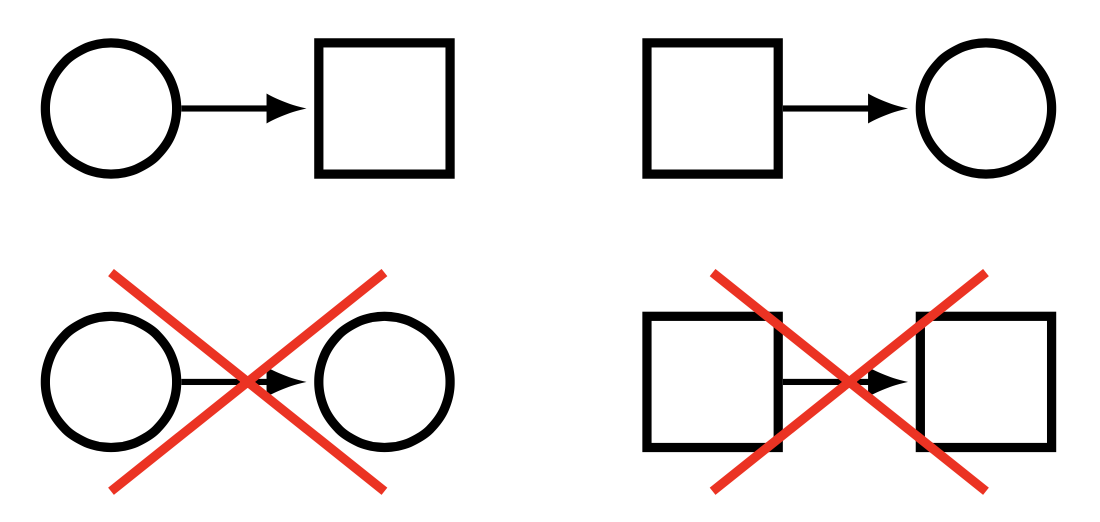
\includegraphics[width=0.4\linewidth]{resources/fluss.png}
	\end{center}

	\bigskip
	\textbf{Marking} -- Assignment of token count to places

	\smallskip
	\begin{minipage}{0.3\textwidth}
		\begin{center}
			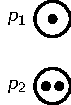
\includegraphics[width=0.3\linewidth]{resources/marking.pdf}
		\end{center}
	\end{minipage}
	\begin{minipage}{0.6\textwidth}
		$ \marking : p_1 \; 2p_2 $ $ \hspace{10pt} \rightarrow $ \emph{multi-set notation}
	\end{minipage}
\end{frame}

\subsection{Petri Net Behavior}

\begin{frame}{Executing Rule}
	\label{frame:execution_rule}
	\textbf{Executing a transition} $ t \in T $ of Petri net $ \pn[=] $\\
	Change token count of places

	\begin{defi}{Activation and Execution of a Transition}{}
		Transition $ t \in T $ of $ \pn[=] $ is \emph{activated} in marking $ \marking $, if
		\vspace{-8pt}
		\begin{align*}
			\forall p \in P : w(p,t) \leq \marking(p)
		\end{align*}
		\vspace{-20pt}

		Notation: $ \marking \xrightarrow{t} $

		If $ \marking \xrightarrow{t} $, \emph{executing} $ t $ in $ \marking $ leads to marking $ \marking[][\prime] $ with
		\vspace{-8pt}
		\begin{align*}
			\forall p \in P : \marking[][\prime](p) = \marking(p) + w(p,t) - w(t,p)
		\end{align*}
		\vspace{-20pt}

		Notation: $ \marking \xrightarrow{t} \marking[][\prime] $
	\end{defi}
	{\centering
	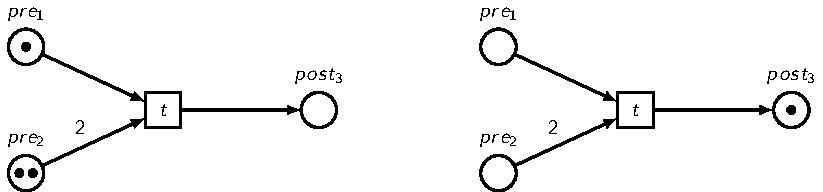
\includegraphics[width=0.8\textwidth]{resources/firing.pdf}
	\par}


\end{frame}

\begin{frame}{Example - PN}
	\begin{beispiel}{Petri net $ \pn[=] $}{}
		\begin{itemize}
			\item[] $ P = \set{sem,crit_1,start_1,idle_1,wait_1,crit_2,start_2,idle_2,wait_2} $
			\item[] $ T = \set{acq_1,rel_1,proc_1,req_1,acq_2,rel_2,proc_2,req_2} $
			\item[] $ \marking[0] : start_1 \; sem \; wait_2 $
		\end{itemize}

		\bigskip
		{\centering
			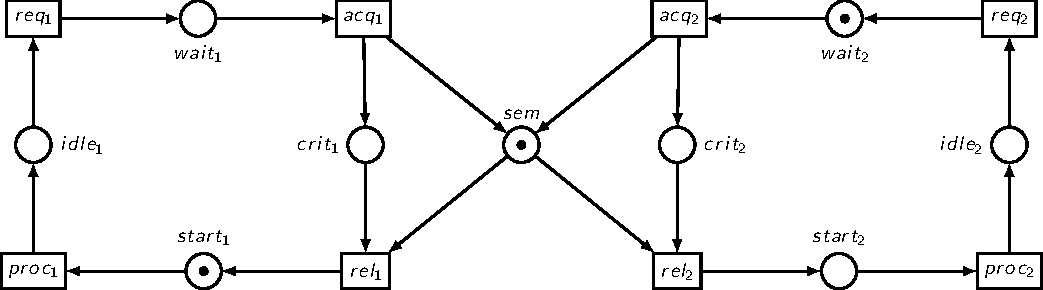
\includegraphics[width=\textwidth]{resources/semaphor.pdf}
			\par}
	\end{beispiel}




\end{frame}

\begin{frame}{State Space}
	\textbf{State Space} generation of Petri net $ \pn[=] $

	\bigskip
	\emph{How?}

	DFS/BFS exploration --  executing activated transitions in a marking

	\begin{defi}{State Space}{}
		The \emph{state space} $ \ss[=] $ of $ \pn[=] $ is a directed, labeled graph, inductively defined as follows: \\
		Base: $ \marking[0] \in V $ \\
		Step: If $ \marking \in V $ and $ \marking \xrightarrow{t} \marking[][\prime] $ for $ t \in T $, then $ (\marking,t, \marking[][\prime]) \in E $ and $  \marking[][\prime] \in V $.
	\end{defi}

	\bigskip
	Similar:
	\begin{itemize}
		\item Labelled Transition System
		\item Kripke structure \cite{clarke_compositional_1989}
	\end{itemize}
\end{frame}

\begin{frame}{Example - SS}
	\vspace{-10pt}
	\begin{beispiel}{State Space $ \ss[=] $ of Petri net $ \pn $}{}
		{\centering
			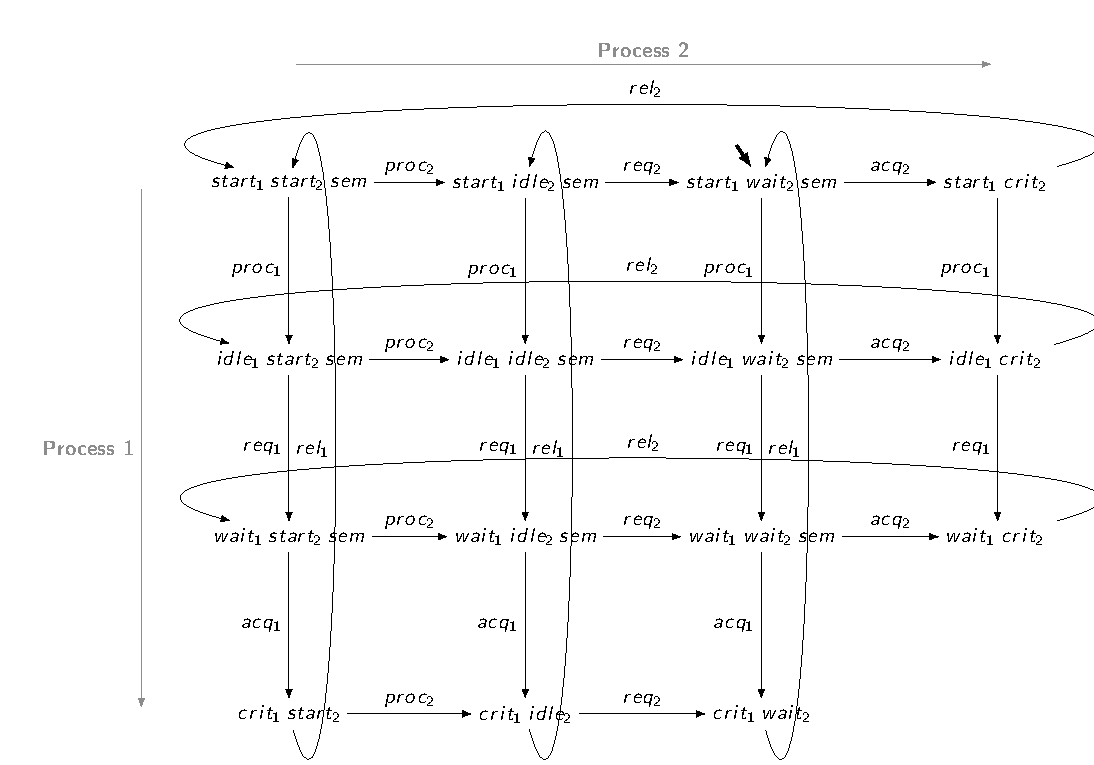
\includegraphics[width=0.8\textwidth]{resources/ss_semaphor.pdf}
			\par}
		with $ \abs{V} = 15 $ and $ \abs{E} = 28 $
	\end{beispiel}

\end{frame}

\subsection{Model Checking with Petri Nets}

\begin{frame}{Pipeline for Petri Nets}
	\centering
	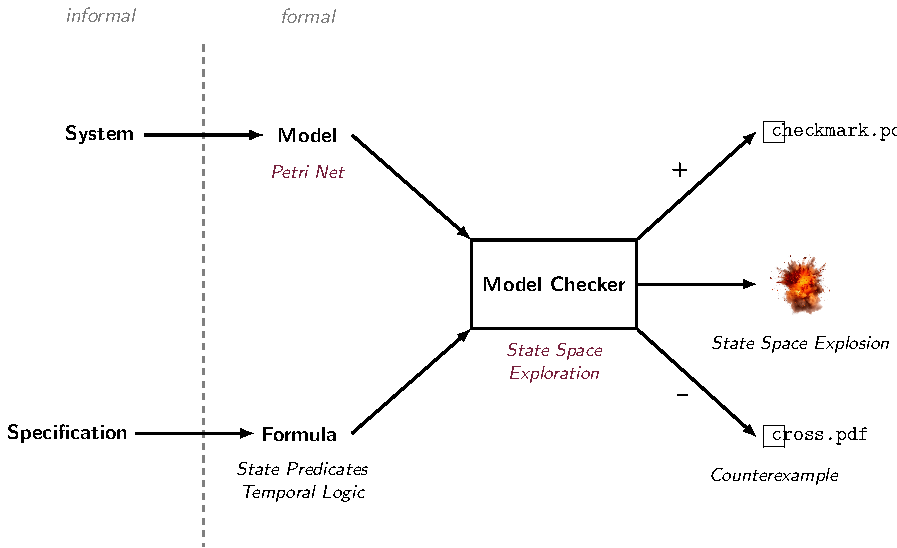
\includegraphics[width=\textwidth]{resources/pipeline_pn.pdf}
\end{frame}

\begin{frame}{Avoiding State Space Explosion}
	\begin{merke}{Size of the State Space}{}
		State space $ \ss $ can become exponentially large in the size of Petri net $ \pn $ (or even infinitely big).
	\end{merke}

	$ \rightarrow $ Avoiding state space explosion by exploiting the Petri net formalism

	\bigskip
	Strong connection between structure and behavior of Petri nets allows

	\medskip

	\begin{enumerate}
		\item \textbf{State Space Reduction Methods} \\
		      $ \rightarrow $ Minimization of the number of explored states
		\item \textbf{Net Structure Analysis} \\
		      $ \rightarrow $ No state space generation
		      (for specific net classes)
	\end{enumerate}
\end{frame}

\subsubsection{State Space Reduction Methods}

\subsubsubsection{Partial Order Reduction}

\begin{frame}{Partial Order Reduction}
	\begin{tabular}{c p{10cm}}
		$ \textbf{Idea} $ & Concurrent actions cannot (de)activate each other         \cite{esparza_unfoldings_2008} \\
		                  & $ \rightarrow $ Independent in their execution order                                     \\
		                  & $ \rightarrow $ State reachable by any permutation of concurrent actions                 \\
		                  & {\centering 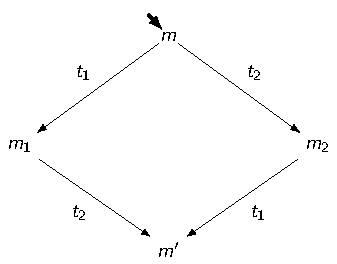
\includegraphics[width=0.2\textwidth]{resources/po.pdf}\par}                 \\
		\textbf{Goal}     & Reduce state space by permutations of concurrent actions                                 \\
		                  &                                                                                          \\
		\bfrightarrow     & \emph{Stubborn Set Method} \cite{valmari_stubborn_1991}                                  \\
		                  & {\small explore only non-concurrent transitions in a marking}                            \\
		                  &                                                                                          \\
		\bfplus           & Enormous reduction esp. in concurrent systems                                            \\
		\bfminus          & Restriction of checkable specifications
	\end{tabular}
\end{frame}

\subsubsubsection{Symmetry}

\begin{frame}{Symmetry}
	\begin{tabular}{c p{12cm}}
		$ \textbf{Idea} $ & Symmetrical structures generate symmetrical behavior                           \\
		                  &                                                                                \\
		$ \textbf{Goal} $ & Reduce state space by symmetrical behavior                                     \\
		                  &                                                                                \\
		\bfrightarrow     & \emph{Symmetry Method} \cite{starke_reachability_1991} \cite{schmidt_how_2000} \\
		                  & {\small Detect symmetric markings by automorphisms of the Petri net and }      \\
		                  & {\small avoid their exploration}                                               \\
		                  &                                                                                \\
		\bfplus           & Enormous reduction esp. in symmetrical systems                                 \\
		\bfminus          & Automorphism = strict mathematical concept allows no deviations                \\
		                  & Restriction of checkable specifications                                        \\
	\end{tabular}
\end{frame}

\subsubsubsection{Coverability}

\begin{frame}{Coverability - General}

	Assume $ \pn[=] $ generates an \emph{infinite} state space

	\bigskip

	% Beipiel
	\begin{tabular}{c p{12cm}}
		$ \textbf{Idea} $ & Identify and abstract infinite Behavior                                     \\
		                  &                                                                             \\
		\textbf{Goal}     & Finite state space                                                          \\
		                  &                                                                             \\
		\bfrightarrow     & \emph{Coverability Graph} \cite{karp_parallel_1969}                         \\
		                  & {\small Detect sequences of infinite sequences of states and abstract them} \\
		                  &                                                                             \\
		\bfplus           & Always finite \cite{karp_parallel_1969}                                     \\
		\bfminus          & Coverability = Abstraction $ \rightarrow $ behavior may be concealed        \\
		                  & Restriction of checkable specifications                                     \\
	\end{tabular}
\end{frame}

\begin{frame}{Coverability - Example I}
	\begin{beispiel}{Petri Net $ \pn $ with unbounded State Space}{}
		\centering
		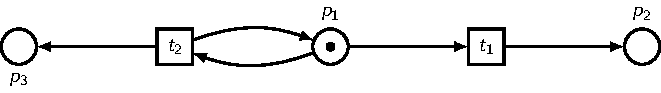
\includegraphics[width=0.8\textwidth]{resources/unbounded.pdf}

		\bigskip
		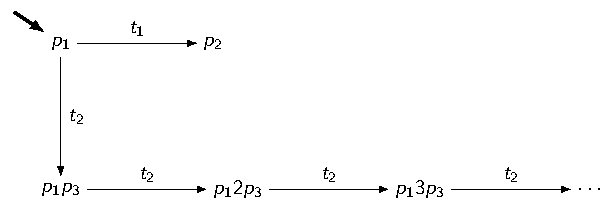
\includegraphics[width=0.8\textwidth]{resources/ss_unbounded.pdf}

		\bigskip
		Number of Tokens on $ p_3 \rightarrow \infty $
	\end{beispiel}
\end{frame}

\begin{frame}{Coverability - Method I}
	\textbf{Coverability Graph} of Petri net $ \pn[=] $

	\medskip

	DFS-Exploration

	\medskip
	Marking $ \marking \rightarrow $ DFS-Stack $ \stack(\marking) $

	= Stack of markings from $ \marking[0] $ to $ \marking $

	\bigskip
	For freshly explored marking $ \marking $ check: $ \exists \marking^* \in \stack(\marking) : \marking^* < \marking $?

	$ \rightarrow $ \emph{$ \marking $ covers a predecessor marking $ \marking^* $?}

	$ \rightarrow $ behavior of $ \marking^* $ would be possible in $ \marking $ as well!

	\medskip
	\emph{Why?}
	\begin{merke}{Monotony of Executing Transitions}{}
		Assume $ \marking \xrightarrow{t} \marking^\prime $ for $ t \in T $ and there exists a marking $ \marking_1 \geq \marking $.\\
		This implies the existence of marking $ \marking_1^\prime \geq \marking^\prime $ with $ \marking_1 \xrightarrow{t} \marking_1^\prime $.
	\end{merke}
\end{frame}

\begin{frame}{Coverability - Method II}
	Assume $ \exists \marking^* \in \stack(\marking) : \marking^* < \marking $.

	$ \rightarrow $ \textbf{Pumping sequence} $ \sigma \in T^*: \marking^* \xrightarrow{\sigma} \marking $


	\medskip
	According to monotony of executing transitions:

	$ \rightarrow $ Pumping sequence $ \sigma $ is executable in $ \marking $, leading to marking $ \marking^\prime > \marking  $

	$ \rightarrow $ Can be repeated infinitely often

	$ \rightarrow $ Infinite sequence of covering markings

	\medskip

	Assume place $ p \in P $ with $ \marking^*(p) < \marking(p) $.

	$ \rightarrow $ Token count on $ p $ grows into the infinite



	\smallskip
	$ \rightarrow $ \contour{black}{$ \omega$} \textbf{-Abstraction} $ \marking(p) \leftarrow \omega $

	\hspace{0.3cm} $ \omega $ = infinitely many tokens

	\begin{satz}{Finite Coverability Graph \cite{karp_parallel_1969}}{}
		The coverability graph of $ \pn $ is finite.
	\end{satz}
\end{frame}

\begin{frame}{Coverability - Example II}

	\begin{beispiel}{Petri Net $ \pn $ with unbounded State Space}{}
		\centering
		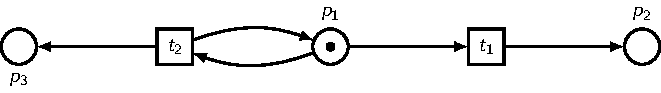
\includegraphics[width=0.9\textwidth]{resources/unbounded.pdf}
		\bigskip
		\begin{minipage}{0.7\textwidth}
			\centering
			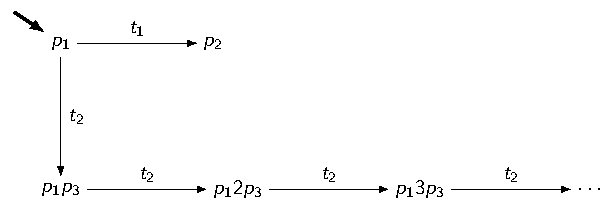
\includegraphics[width=\textwidth]{resources/ss_unbounded.pdf}
		\end{minipage}
		\begin{minipage}{0.25\textwidth}
			\centering
			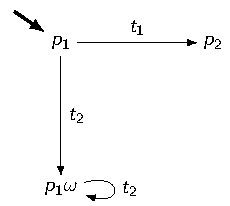
\includegraphics[width=\textwidth]{resources/ss_unbounded_bounded.pdf}
		\end{minipage}
	\end{beispiel}
\end{frame}

\section{Modular Petri Nets}

\begin{frame}[noframenumbering,plain]{Section Page}
	\sectionpage
\end{frame}

\begin{frame}{Compositional Systems}
	Compositional System = Composition of interacting components

	\bigskip

	\textbf{Principle of Locality} Cause and effect of actions are local

	$ \rightarrow $ Component behavior mostly independent of another

	\bigskip
	\textbf{Principle of Compositionality} \cite{frege1892} System behavior deducible from components behavior and the rules of their interaction

	$ \rightarrow $ System behavior = synchronized component behavior

	$ \rightarrow $ Component behavior restricted in the context of the composition
	\bigskip


	\emph{Interesting for Model Checking!}

	\smallskip
	Compositional/Modular Verification --  \cite{clarke_compositional_1989} \cite{shurek1990modular}

	\smallskip
	... for Petri Nets -- \cite{notomi_hierarchical_1994} \cite{donatelli_kronecker_2001} \cite{christensen_modular_2000} \cite{latvala_ltl_2004} \cite{gaede_modular_2024} \cite{gaede_automatic_2024} \cite{zech_verifying_2024} \cite{wallner2026coverability}
\end{frame}

\begin{frame}{General}
	Modeling formalism for compositional systems

	\medskip
	Implicit representation of a Petri net by components and interaction rules

	\begin{defi}{Module, Modular Petri Net \cite{gaede_modular_2024}}{}
		A \emph{module} is a Petri net $ \pn[=] $ such that \\
		$ T = \internals \cup \interfaces $, where
		\begin{itemize}
			\item  $ \internals $ is a set of internal transitions, and
			\item  $ \interfaces $ is a set of interface transitions.
		\end{itemize}
		\medskip
		A \emph{modular Petri net} is a tuple $ \ms[=] $, where
		\begin{itemize}
			\item $ \modules[=] $ is a set of disjoint modules.
			\item $ \synchronizations \subseteq (\interfaces[1] \cup \set{\epsilon}) \times \dotsc \times (\interfaces[\modulecard] \cup \set{\epsilon}) $ is a set of \emph{synchronizations}.
		\end{itemize}
	\end{defi}
\end{frame}

\begin{frame}{Example - MPN}
	\begin{beispiel}{Modular Petri Net $ \ms[=] $}{}
		with $ \modules = \set{\module{1},\module{2},\module{3}} $ and $ \synchronizations = \set{\synchronization_1,\synchronization_2} $, where
		\vspace{-10pt}
		\begin{multicols}{2}
			\begin{itemize}
				\item[] $ \synchronization_{acq_1} = [acq_1,acq_3] $
				\item[] $ \synchronization_{rel_1} = [rel_1,rel_3] $
				\item[] $ \synchronization_{acq_2} = [acq_3,acq_2] $
				\item[] $ \synchronization_{rel_2} = [rel_3,rel_2] $
			\end{itemize}
		\end{multicols}

		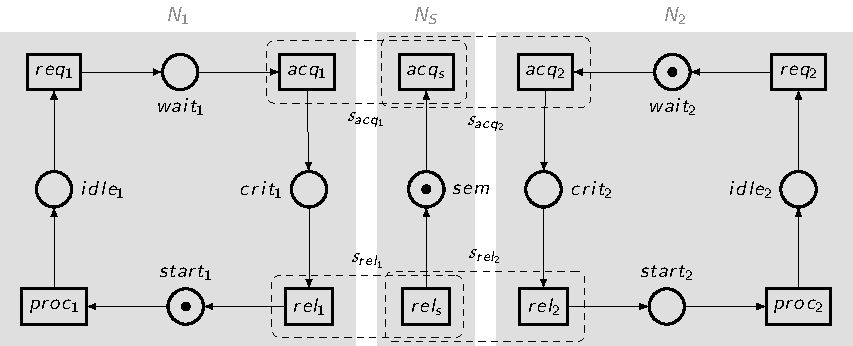
\includegraphics[width=\textwidth]{resources/msemaphor.pdf}

	\end{beispiel}
\end{frame}

\subsection{Modular Petri Net Behavior}

\begin{frame}{Module Behavior I}

	\begin{merke}{Module Behavior}{}
		Behavior of module $ \module{j} \in \modules $ is defined locally and independent of the other modules of the modular Petri net $ \ms[=] $.
	\end{merke}

	\bigskip
	\textbf{Local Marking} -- Assignment of token count to module places

	\begin{align*}
		\localmarking{j}: P_j \rightarrow \nat
	\end{align*}


	\textbf{Executing a module transition} $ t \in \internals[j] \cup \interfaces[j] $ of $ \module{j} \in \modules $

	Change token count of module places

	Activation $ \localmarking{j} \xrightarrow{t} $ and execution
	$ \localmarking{j} \xrightarrow{t} \localmarking{j}^\prime $ on local markings $ \localmarking{j}, \localmarking{j}^\prime $ are defined similar to transitions of a Petri net (cf. Slide~\ref{frame:execution_rule}).
\end{frame}

\begin{frame}{Module Behavior Restriction}
	\begin{merke}{Module Composition restricts Module Behavior}{}
		No restriction:
		\textbf{Internal transition}

		= module-internal behavior

		$ \rightarrow $ Individual execution

		\bigskip
		Restriction:
		\textbf{Interface transition}

		= interaction behavior

		$ \rightarrow $ Execution of $ t \in \interfaces[j] $ only in the context of activated synchronization $ \synchronization \in \synchronizations $, where $ \synchronization[j] = t $.
	\end{merke}
\end{frame}

\begin{frame}{Synchronization}

	\textbf{Marking} -- Concatenation of local markings \\
	\begin{align*}
		\concatmarking
	\end{align*}
	where $ \localmarking{j} $ is a local marking of module $ \module{j} \in \modules $.

	\bigskip
	\textbf{Executing a synchronization} $ \synchronization \in \synchronizations $

	Change number of tokens on the module places globally \\

	\begin{defi}{Activation and Execution of a Synchronization}{}
		\smallskip
		Synchronization $ \synchronization \in \synchronizations $ is \emph{activated} in marking $ \concatmarking $, if $ \localmarking{j} \xrightarrow{\synchronization[j]} $ for $ \synchronization[j] \in \interfaces[j] \cup \set{\epsilon}$ for each module $ \module{j} \in \modules $.

		\smallskip
		\emph{Execution} of activated synchronization $ \synchronization \in \synchronizations $ in marking $ \concatmarking $ leads to marking $ \concatmarking[\prime] $, where $ \localmarking{j} \xrightarrow{\synchronization[j]} \localmarking{j}^\prime $.

		\smallskip
		Note that:  $ \localmarking{j} \xrightarrow{\epsilon} \localmarking{j} $ for every local marking $ \localmarking{j} $.
	\end{defi}
\end{frame}

\begin{frame}{Modular State Space Generation}
	\textbf{Modular State Space} generation of modular Petri net $ \ms[=] $

	\bigskip
	\emph{How?}

	Synchronized exploration of the module behavior

	\medskip

	\begin{defi}{Modular State Space \cite{gaede_modular_2024}}{}
		The \emph{modular state space} $ \crazy{R} = [\set{\lss{j}[=] \mid \module{j} \in \modules}, R_{\synchronizations}=[V_{\synchronizations},E_{\synchronizations}]] $ is a tuple, where
		\begin{itemize}
			\item $ \lss{j}[=] $ is the \emph{local state space} of $ \module{j} \in \modules $\\
			      $ \rightarrow $ module behavior (internal + interface)
			\item $ R_{\synchronizations}=[V_{\synchronizations},E_{\synchronizations}] $ is the \emph{synchronization graph}\\
			      $ \rightarrow $ synchronization behavior
		\end{itemize}
	\end{defi}

\end{frame}

\begin{frame}{Modular State Space Generation}
	Exhaustively repeat

	\begin{enumerate}
		\item[i.] Exhaustively explore local behavior \\
		      \begin{itemize}
			      \item module internal behavior $ \rightarrow \set{\lss{j}[=]} $
		      \end{itemize}
		      $ \rightarrow $ parallelizable
		\item[ii.] Execute a synchronization when activated \\
		      \begin{itemize}
			      \item module interface behavior $ \rightarrow \set{\lss{j}[=]} $
			      \item synchronization $ \rightarrow  R_{\synchronizations}=[V_{\synchronizations},E_{\synchronizations}] $
			      \item[] \textbf{Base:} abstraction of module behavior between synchronizations
			            $ \rightarrow $ \emph{segment abstraction}
			            \begin{defi}{Segment, Generator}{}
				            A \emph{segment} $ \segment[j] $ is internal-only behavior of a module $ \module{j} \in \modules $ based on set of local markings $ \generator[j] $ (\emph{Generator}).

				            Formally: $ \segment[j]= \acc{\generator[j]} = \set{\localmarking{j}^\prime \mid \localmarking{j} \xrightarrow{\sigma} \localmarking{j}^\prime, \localmarking{j} \in \generator[j], \sigma \in \internals[j]}$
			            \end{defi}
		      \end{itemize}
		      $ \rightarrow $ may activate further local behavior
	\end{enumerate}
\end{frame}

\begin{frame}{Segment Abstraction}
	Building the \textbf{synchronization graph} $ R_{\synchronizations}=[V_{\synchronizations},E_{\synchronizations}] $:

	{\centering
	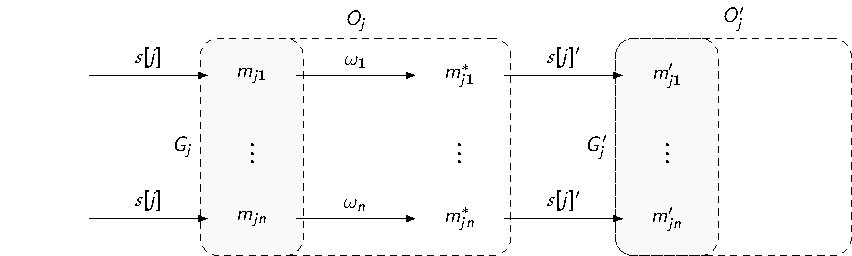
\includegraphics[width=0.8\textwidth]{resources/segment.pdf}
	\par}

	\begin{itemize}
		\item Collect internal-only behavior of module $ \module{j} \in \modules $ between synchronizations $ \rightarrow $ segment $ \segment[j] $
		\item[] Initial segment:
		      $ \segment[j] = \acc{\set{\localmarking{j0}}} $
		\item Vertex $ v \in V_{\crazy{S}} :$ $ \modulecard $-tuple of segments
		      $ v = \segment[1] \dotsc \segment[\modulecard] $
		\item[]
		      $ \rightarrow $ Abstraction of modular Petri net behavior
		\item Edge $ (v,\synchronization,v^\prime) \in E_{\crazy{S}} :$ Synchronization $ \synchronization \in \synchronizations $
		\item[] Successor vertex $ v^\prime = \segment[1]^\prime \dotsc \segment[\modulecard]^\prime $, where $ \segment[j]^\prime = \acc{\generator[j]^\prime} $ for $ \generator[j]^\prime = \set{\localmarking{j}^\prime \mid \localmarking{j} \xrightarrow{\synchronization[j]} \localmarking{j}^\prime, \localmarking{j} \in \segment{j}} $
	\end{itemize}

\end{frame}

\begin{frame}{Example - MSS I}
	\begin{beispiel}{Modular State Space}{}
		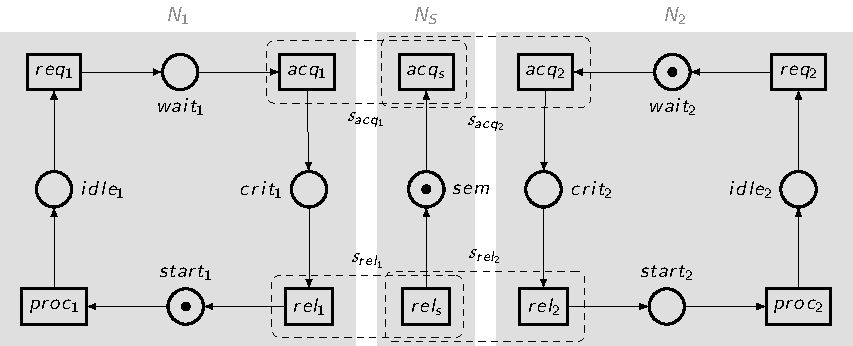
\includegraphics[width=\textwidth]{resources/msemaphor.pdf}
	\end{beispiel}
\end{frame}

\begin{frame}{Example - MSS II}
	\vspace{-0.3cm}
	\begin{beispiel}{Modular State Space}{}
		\centering
		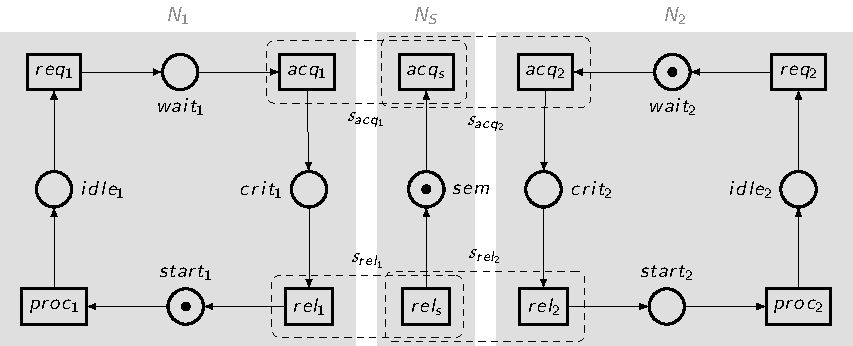
\includegraphics[width=0.5\textwidth]{resources/msemaphor.pdf}

		\begin{minipage}{0.25\textwidth}
			\centering
			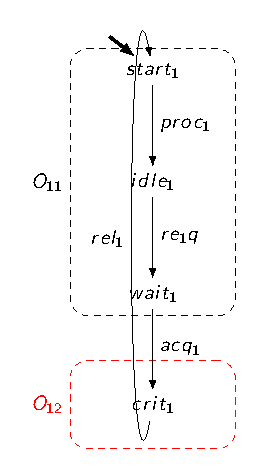
\includegraphics[width=0.9\textwidth]{resources/lss1.pdf}
		\end{minipage}
		\begin{minipage}{0.45\textwidth}
			\centering
			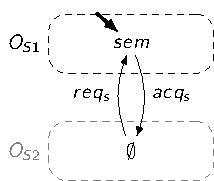
\includegraphics[width=0.4\textwidth]{resources/lsss.pdf}

			\bigskip
			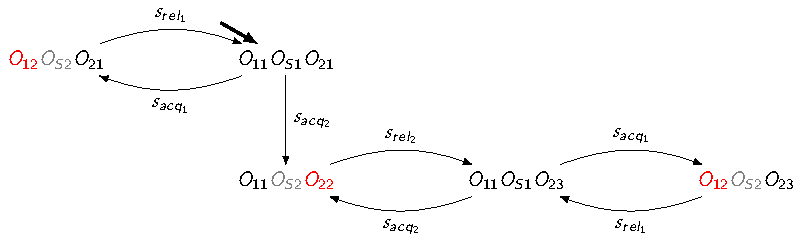
\includegraphics[width=\textwidth]{resources/sg.pdf}
		\end{minipage}
		\begin{minipage}{0.25\textwidth}
			\centering
			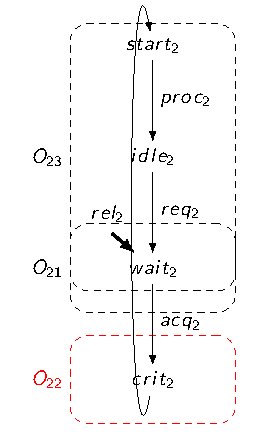
\includegraphics[width=0.9\textwidth]{resources/lss2.pdf}
		\end{minipage}
	\end{beispiel}
\end{frame}

% \begin{frame}{75 Philosophers Example}
% 	% TODO
% \end{frame}

\begin{frame}{SS vs. MSS}

	\begin{merke}{Modularization}{}
		Every Petri net $ \pn[=] $ can be transformed into a modular Petri net.
	\end{merke}
	How? $ \rightarrow $ \cite{gaede_automatic_2024}

	\bigskip

	\begin{satz}{Marking Equivalence \cite{gaede_modular_2024}}{}
		Let Petri net $ \pn[=] $ given in form of a modular Petri net $ \ms[=] $.\\
		Let $ \ss[=] $ be the state space of $ \pn $ and $ \crazy{R} = [\set{\lss{j}[=] \mid \module{j} \in \modules}, R_{\synchronizations}=[V_{\synchronizations},E_{\synchronizations}]]$ be its modular state space.\\
		It holds that marking $ \marking \in V $
		if and only if there exists a vertex $ \segment[1] \dotsc \segment[\modulecard] \in V_{\synchronizations} $ such that $ \marking \in \segment[1] \times \dotsc \times \segment[\modulecard] $.
	\end{satz}
	$ \rightarrow $ Modular state space contains the exact set of states of $ \pn $ \smiley{}
\end{frame}

\subsection{Model Checking with Modular Petri Nets}

\begin{frame}{Model Checking with Modular Petri Nets}

	Modular state space contains the exact set of states of $ \pn $

	$ \rightarrow $ State explosion problem remains \frownie{}

	\bigskip
	\emph{Why modular Petri nets?}

	\medskip
	Exploiting the modular Petri net formalism by
	\begin{enumerate}
		\item \textbf{Heterogeneity of the Modules}\\
		      $ \rightarrow $ Module-specific state local state space generation
		\item \textbf{Instantiation}\\
		      $ \rightarrow $ Reusing local markings
		\item \textbf{Abstraction}\\
		      $ \rightarrow $ Model checking only on the synchronization graph
	\end{enumerate}
	to counteract state explosion problem
\end{frame}

\subsubsection{Heterogeneity of Modules}

\begin{frame}{General}
	\begin{merke}{Recall from part 2}{}
		\begin{itemize}
			\item success of state space reduction methods depends on Petri net structure
			\item state space generation avoidable for distinct Petri net classes only
		\end{itemize}
	\end{merke}

	\bigskip
	\begin{tabular}{r p{10cm}}
		$ \textbf{Idea} $ & Methods more effective for single modules than for the entire Petri net        \\
		                  &                                                                                \\
		$ \textbf{Goal} $ & local state space exploration tailored to the modules                          \\
		                  & $\rightarrow $ reduced segments
		\\
		                  &                                                                                \\
		$ \textbf{But} $  & Explore sufficient behavior to maintain marking equivalence to the state space \\
	\end{tabular}
\end{frame}

\begin{frame}{General II}
	\emph{Sufficient behavior to maintain marking equivalence?}

	\begin{merke}{Requirement for Reduced Segment}{}
		A segment must be completely deducible from the reduced segment
	\end{merke}

	\bigskip
	More precisely:

	\smallskip
	Segment $ \segment{j}^\prime  $ evolves from executing $ \synchronization[j]  $ of synchronization $ \synchronization \in \synchronizations $ in segment $ \segment{j} $

	\begin{center}
		$ \downarrow $
	\end{center}

	For any synchronization $ \synchronization \in \synchronizations $:
	Local marking $ \localmarking{j} \in \segment{j} $
	with $ \localmarking{j} \xrightarrow{\synchronization[j]} $ should be deducible from reduced segment $ \segment[j]^* $ to guarantee completeness of $ \segment{j}^\prime $ exploration
\end{frame}

\begin{frame}{Heterogenous Modules}

	Assume segment $ \segment[j] $ with generator $ \generator[j] \subseteq \segment[j] $ of module $ \module{j} \in \modules $.

	\medskip
	Next: Synchronization $ \synchronization \in \synchronizations $

	\medskip
	Build reduced segment $ \segment[j]^* $ if the module is

	\medskip
	\begin{tabular}{r p{8cm}}
		\textbf{conflict-free}    & with single-element stubborn sets                                                                              \\
		\textbf{concurrency-free} & $ \segment[j]^* = \generator[j]$                                                                               \\
		                          & local marking $ \localmarking{j} \in \segment[j] $ with $ \localmarking{j} \xrightarrow{\synchronization[j]} $ \\
		                          &
		= Solution of an ILP                                                                                                                       \\
		                          & NP-complete, but great tool support \smiley                                                                    \\
		                          & = Solution of a maximum flow problem       \cite{wallner2024state}                                             \\

		\textbf{acyclic}
		                          & $ \segment[j]^* = \generator[j]$                                                                               \\
		                          & + linear algebra \cite{schultz2024utilization}                                                                 \\
		                          &                                                                                                                \\
		\textbf{unbounded}        & modular coverability \cite{wallner2026coverability}
	\end{tabular}

\end{frame}

\subsubsubsection{Unbounded Modules}

\begin{frame}{Unbounded Modules I}
	\begin{merke}{Recall from Part 2}{}
		Unbounded Petri nets $ \rightarrow $ DFS-Stack $ \stack(\marking) $ for marking $ \marking $ to identify unbounded behavior with pumping sequences:
		\begin{align*}
			\exists \marking^* \in \stack(\marking) \text{ with } \marking^* \xrightarrow{\sigma} \marking \text{ for } \sigma \in T^* \text{ such that } \marking^* < \marking?
		\end{align*}
	\end{merke}

	\medskip

	In the modular state space:

	Local state spaces $ \rightarrow $ local parts of the pumping sequence (\textbf{local pumping sequences})

	\medskip
	\textbf{Good:}
	\begin{satz}{Projection of Pumping Sequence \cite{wallner2026coverability}}{}
		Pumping sequence $ \sigma \in (\internals \cup \synchronizations)^* $ $ \Rightarrow \exists $ selection $ (\sigma_1,\dotsc,\sigma_\modulecard)$, of local pumping sequences $ \sigma_j \in (\internals[j] \cup \interfaces[j])^* $ that composes to $ \sigma $.
	\end{satz}
\end{frame}

\begin{frame}{Example Combination}
	\textbf{Not So Good:}
	Not every selection of local pumping sequences composes to an actual pumping sequence \frownie

	\begin{beispiel}{}{}
		\begin{minipage}{0.3\textwidth}
			\centering
			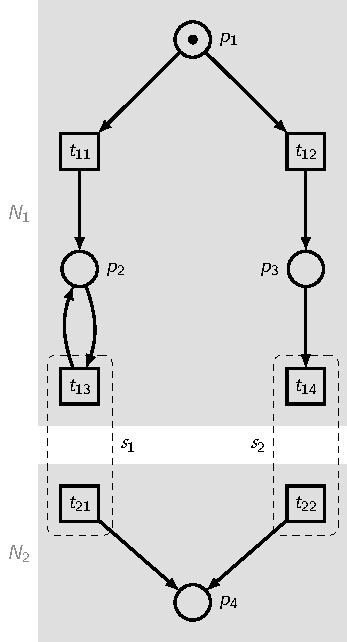
\includegraphics[width=0.9\textwidth]{resources/unbounded_selection}
		\end{minipage}
		\begin{minipage}{0.32\textwidth}
			\centering
			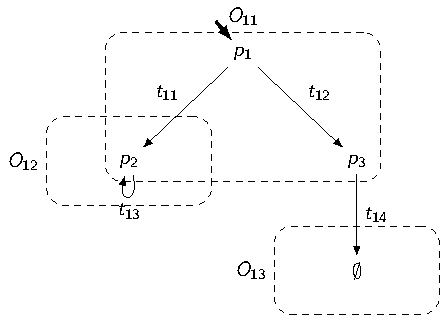
\includegraphics[width=\textwidth]{resources/unbounded_lss1.pdf}

			\bigskip
			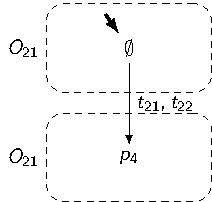
\includegraphics[width=0.7\textwidth]{resources/unbounded_lss2.pdf}
		\end{minipage}
		\begin{minipage}{0.3\textwidth}
			\centering
			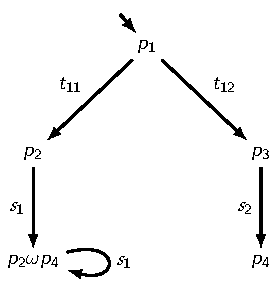
\includegraphics[width=\textwidth]{resources/unbounded_cg.pdf}
		\end{minipage}



	\end{beispiel}
\end{frame}

\begin{frame}{Unbounded Modules I}
	\begin{merke}{Composable Local Pumping Sequences}{}
		A selection of local pumping sequences needs to align in the succession of occurring synchronizations.
	\end{merke}

	$ \rightarrow $ Information from the synchronization graph necessary
	\medskip

	\textbf{Bad:}
	Combinatorial effort!

	\medskip
	{\small

		Assume synchronization graph vertex $ v = \segment[1] \dotsc \segment[\modulecard] $ and marking $ \marking \in  \segment[1] \times \dotsc \times \segment[\modulecard] $ such that $ \concatmarking $.

		\medskip
		For $ \localmarking{j} $: $ \Sigma_j \subseteq (\internals[j] \cup \interfaces[j])^* $ = set of local pumping sequences

		($ \sigma_j \in \Sigma_j $: $ \localmarking{j}^* \xrightarrow{\sigma_j} \localmarking{j} $ such that $ \localmarking{j}^* < \localmarking{j} $)

		\medskip
		$ \rightarrow $ For $ \concatmarking $: check if $ (\sigma_1,\dotsc,\sigma_\modulecard) \in \Sigma_1 \dotsc \Sigma_\modulecard $ aligns in their succession of synchronizations and composes to an actual pumping sequence $ \sigma $ from some marking $ \marking^* < \marking $.}
\end{frame}

\begin{frame}{Unbounded Modules I}
	\textbf{Good News I:} Segments and generators are useful to overcome combinatorial effort \smiley

	\begin{defi}{Generator Marking}{}
		Let $ v = \segment[1] \dotsc \segment[\modulecard] $ be a synchronization graph vertex, where $ \generator[j] $ is the generator of $ \segment[j] $ for module $ \module{j} \in \modules $.

		Marking $ \marking_g \in \generator[1] \times \dotsc \times \generator[\modulecard] $ is a \emph{generator marking}.
	\end{defi}

	% Assume synchronization graph vertex $ v = \segment[1] \dotsc \segment[\modulecard] $, where $ \generator[j] $ is the generator of $ \segment[j] $ for module $ \module{j} \in \modules $.

	% Assume marking $ \marking \in  \segment[1] \times \dotsc \times \segment[\modulecard] $ such that $ \concatmarking $.

	\begin{satz}{Generator Marking Pumping Sequences \cite{wallner2026coverability}}{}
		Pumping sequence $ \sigma \in (\internals \cup \synchronizations)^* $ such that $ \marking^* \xrightarrow{\sigma} \marking $ for $ \marking^* < \marking $ implies a pumping sequence $ \sigma^\prime \in \internals \cup \synchronizations $ such that $ \marking_g^* \xrightarrow{\sigma^\prime} \marking_g $ for $ \marking_g^* < \marking_g $, where $ \marking_g^*, \marking_g $ are generator markings such that
		\begin{itemize}
			\item $ \marking^* \xrightarrow{} \marking_g^* $
			\item $ \marking \xrightarrow{} \marking_g $
		\end{itemize}
	\end{satz}
\end{frame}

\begin{frame}{Figure Shifting}
	Proof Sketch:

	\bigskip
	{\centering
		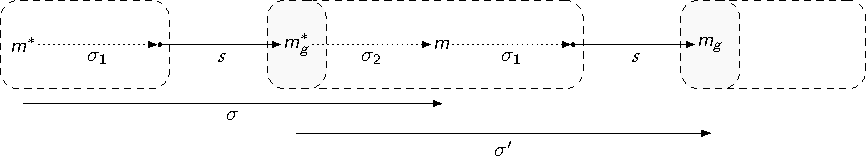
\includegraphics[width=\textwidth]{resources/sequece_shifting.pdf}
		\par}

	Assume

	Pumping sequence $ \sigma = \sigma_1 \synchronization \sigma_2 $ for $ \sigma_1,\sigma_2 \in \internals^* $, $ \synchronization \in \synchronizations : \marking^* \xrightarrow{\sigma} \marking $.
	\smallskip
	$ \marking^* < \marking $.

		{$ \Downarrow $}

	Sequence $ \sigma_1 \synchronization $ executable in $ \marking $.

		{$ \Downarrow $}

	Pumping sequence $ \sigma^\prime = \sigma_2 \sigma_1 \synchronization $ from $ \marking_g^* $ to $ \marking_g $.

	\bigskip
	(extendable for sequences with > 1 synchronizations)
\end{frame}

\begin{frame}{Internal-Only Pumping Sequences}
	\textbf{Good News II:} Internal-Only Pumping Sequences directly detectable in the local state space \smiley


	\begin{defi}{Projection of Sequences}{}
		For sequence $ \sigma \in \internals^* $, let $ \pi_j(\sigma) \in \internals[j]^* $ be the \emph{projection} of $ \sigma $ to module $ \module{j} \in \modules $, such that for transition $ t \in \sigma $, it holds that $ t \in \pi_j(\sigma) $ if and only if $ t \in \internals[j] $.
	\end{defi}

	\begin{satz}{Internal-Only Pumping Sequences \cite{wallner2026coverability}}{}
		Internal-only pumping sequence $ \sigma \in \internals^*: m^* \xrightarrow{\sigma} m' $ for $ m^* \leq m' $, iff local pumping sequence
		$ \pi_j(\sigma) \in \internals[j]^*: \pi_j(m^*) \xrightarrow{\pi_j(\sigma)} \pi_j(m') $ for module $ \module{j} \in \modules $.
	\end{satz}
\end{frame}

\subsubsection{Instantiation}

\begin{frame}{Instantiation}

	\begin{tabular}{r p{10cm}}
		$ \textbf{Idea} $ & Modules = \textbf{Instances} of the same Petri net with different initial markings \\
		                  & $ \rightarrow $ more robust than the symmetry method \cite{schmidt_how_2000}       \\
		$ \textbf{Goal} $ & Explore local state space only once                                                \\
	\end{tabular}

	\medskip
	\begin{beispiel}{Instantiation}{}
		\centering
		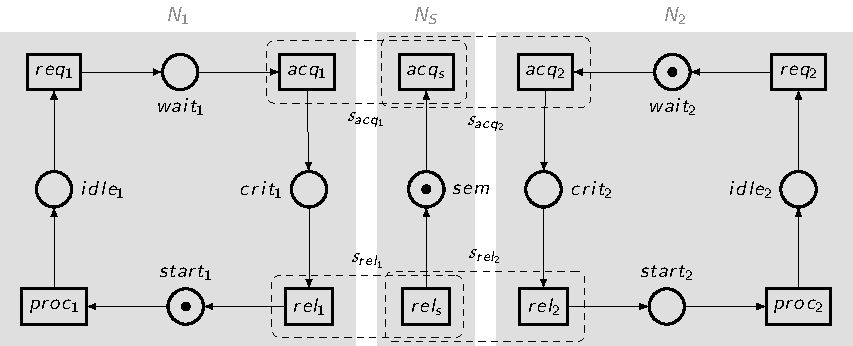
\includegraphics[width=\textwidth]{resources/msemaphor.pdf}
	\end{beispiel}
\end{frame}

\begin{frame}{Example - Instantiation}
	\vspace{-0.4cm}
	\begin{beispiel}{Instantiation}{}
		\begin{minipage}{0.3\textwidth}
			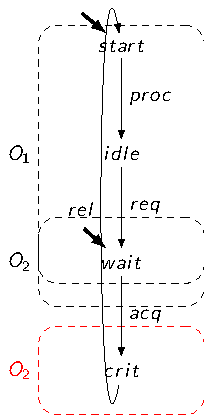
\includegraphics[width=0.6\textwidth]{resources/i_lss.pdf}

			\bigskip
			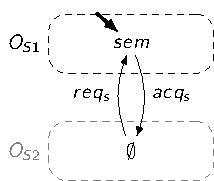
\includegraphics[width=0.6\textwidth]{resources/lsss.pdf}
		\end{minipage}
		\begin{minipage}{0.7\textwidth}
			\centering
			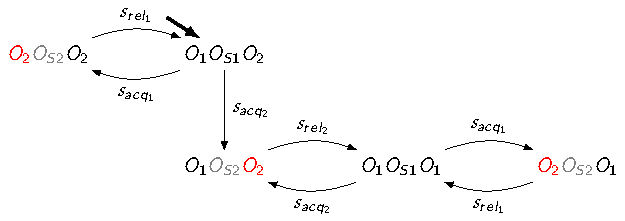
\includegraphics[width=\textwidth]{resources/i_sg.pdf}
		\end{minipage}

		\bigskip
		{\small $ \rightarrow 11 $ vertices \& $ 13 $ edges vs. $ 15 $ vertices and $ 17 $ edges without instantiation}
	\end{beispiel}
\end{frame}

\subsubsection{Abstraction}

\begin{frame}{General}
	\begin{tabular}{r p{10cm}}
		$ \textbf{Idea} $ & Synchronization graph = Abstraction of the state space                 \\
		                  & $ \rightarrow $ Abstract model checking with the synchronization graph \\
	\end{tabular}

	\begin{merke}{Abstract Model Checking and Behavioral Equivalences}{}
		Logic of the formula $ \rightarrow $ necessary \emph{behavioral equivalence} between the system and its abstraction.
	\end{merke}

	\begin{tabular}{r p{6cm}}
		State Predicates                                  & \textbf{State Equivalence}               \\
		(Propositional Logic)                             & $ \rightarrow $ same set of states       \\
		Linear Time Logic \cite{pnueli_temporal_1977}     & \textbf{Trace Equivalence}               \\
		                                                  & $ \rightarrow $ same set of executions   \\
		Branching Time Logic \cite{ben-ari_temporal_1981} & \textbf{Bisimulation}                    \\
		                                                  & $ \rightarrow $ same branching structure
	\end{tabular}
	cf. \cite{glabbeek_linear_2001}
\end{frame}

\begin{frame}{For MSS}
	\emph{What can we check in the synchronization graph?}

	\bigskip
	\begin{tabular}{r p{6cm}}
		State Predicates      & 
\includegraphics[width=0.03\textwidth]{resources/checkmark.pdf} \\
		(Propositional Logic) & cf. Thm:Marking Equivalence                                     \\
		                      &                                                                 \\
		Linear Time Logic     & 
\includegraphics[width=0.03\textwidth]{resources/checkmark.pdf} \\
		                      & cf. \cite{zech_verifying_2024}                                  \\
		                      &                                                                 \\
		Branching Time Logic  & 
\includegraphics[width=0.03\textwidth]{resources/cross.pdf}     \\
		                      & $ \rightarrow $ Refinement necessary!                           \\
		                      & cf. \cite{zech_verifying_2024}
	\end{tabular}


\end{frame}

\subsection{Conclusion}

\begin{frame}{Conclusion}

	\textbf{Modular Petri Nets}

	\begin{itemize}
		\item[=] modelling formalism for (compositional) systems based on Petri nets
	\end{itemize}

	\medskip
	\textbf{Model Checking for Modular Petri Nets}

	Base: Modular state space -- marking equivalent to state space

	\smallskip
	Effective by exploiting
	\begin{itemize}
		\item Heterogeneity of the modules
		\item Instantiation
		\item Abstraction
	\end{itemize}

	\medskip
	\textbf{Future Work}

	\begin{itemize}
		\item Verification-optimal automatic modularization
		\item Inclusion of symbolic model checking methods, e.g. BDDs
		\item State space reduction methods for the synchronization graph
	\end{itemize}
\end{frame}

\section{References}

\begin{frame}[allowframebreaks]{References}
	\bibliographystyle{amsalpha}
	\bibliography{literature.bib}
\end{frame}

\end{document}